\documentclass[a4paper,12pt]{article}

\usepackage{fancyhdr}
\usepackage{lastpage}
\usepackage{amsmath, amssymb, amsthm}
\usepackage{bm}
\usepackage{wrapfig}
\usepackage{braket}
\usepackage{mathtools}
\usepackage[noend, linesnumbered]{algorithm2e}
\SetKwComment{Comment}{$\triangleright$\ }{}
\RestyleAlgo{ruled}
\usepackage[skip=2pt]{parskip}  
\usepackage{tikz}
\usetikzlibrary{arrows.meta, positioning}
\usepackage[edges]{forest} % Para a árvore de busca


% ---- PREENCHA ----
\newcommand{\Lista}{1}
\newcommand{\Nome}{Isis Ardisson Logullo}
\newcommand{\NUSP}{7577410}
% -----------------------------

\newcommand{\N}{\mathbb{N}}
\newcommand{\bigO}[1]{\ensuremath{\mathcal{O}(#1)}}

\pagestyle{fancy}
\fancyhf{}
\fancyhead[L]{\Nome}
\fancyhead[R]{NUSP \NUSP}
\fancyfoot[L]{Lista \Lista}
\fancyfoot[C]{MAC0425}
\fancyfoot[R]{Página \thepage\ de \pageref{LastPage}}

\begin{document}

\section*{Exercício 1}

Nesta disciplina, adotamos a noção de “agente inteligente” proposta
pelo livro AIMA de Russel e Norvig.\\

\textbf{PARTE A}. Defina essa noção em termos de \textit{pensar} ou \textit{agir} e \textit{racional} ou \textit{humano}.\\

\textbf{PARTE B}. Explique como podemos verificar se um agente computacional é inteligente
ou não.\\

\subsection*{Resposta:}

\bigskip

A) O agente inteligente tem o foco no comportamento externo, baseado numa ação e não em processos internos de pensamento ligados a cognição. O agente é definido pelo que faz: o ambiente alimenta seus sensores e ele retorna uma ação com seus atuadores.

O objetivo do agente não é imitar o comportamento humano, mas sim a racionalidade. Um agente inteligente é aquele que age para alcançar o melhor resultado possível ou o melhor resultado esperado, dadas as informações que possui.
Um agente inteligente é um sistema que percebe seu ambiente e toma ações que maximizam suas chances de sucesso.\\

B) Para verificar se um agente computacional é inteligente, medimos sua racionalidade técnica e desempenho.
Essa medida é feita através de um critério de sucesso. O mapeamento de percepção do agente é feito pela verificação da  escolha da ação que maximiza o desempenho com base na sua sequência de percepções e no seu conhecimento prévio.

Diferente do teste de Turing, que foca na capacidade de se passar por humano, a verificação dos agentes é funcional. Se ele escolhe consistentemente o melhor resultado ele é considerado racional e, portanto, inteligente.


\newpage
\section*{Exercício 3}

Um agente do tipo consulta-tabela (lookup table) olha uma tabela
do tipo percepção/ação (em oposição a um agente que raciocina ou que resolve
problemas, como por exemplo um agente de busca). Esse tipo de agente pode
enfrentar algumas dificuldades com relação à sua capacidade de resolver problemas e
seu desempenho. Dificuldades também podem surgir durante a fase de projeto. Liste
quais podem ser essas dificuldades.

\subsection*{Resposta:}

\bigskip

Um agente de consulta-tabela armazena uma ação para cada sequência de percepções possíveis. Por conta desse comportamento, enfrenta algumas dificuldades:

\begin{itemize}
	\item Tabela muito grande: o número de sequências de percepções possíveis cresce exponencialmente, mesmo para casos simples.
	\item Tempo de construção: é necessário definir manualmente a ação correta para cada combinação possível de entrada, o que é humanamente impossível em ambientes complexos.
	\item Falta de autonomia: não "aprende" nem se adapta, se o ambiente mudar ligeiramente e gerar uma percepção que não está na tabela, ele não saberá o que fazer. Depende inteiramente do conhecimento prévio inserido.
	\item Desperdício de memória: armazenar todas as combinações exige muito espaço na memória e o custo disso seria altíssimo.
	\item Não funciona com ambientes dinâmicos: não consegue prever consequências de ações que não foram explicitamente mapeadas.
\end{itemize}


\newpage
\section*{Exercício 4}

Explique as seguintes categorizações dos algoritmos de busca:\\
(a) Busca informada e Busca não-informada\\
(b) Busca em árvore e busca em grafo\\
(c) Busca por planejamento de ações e Busca por identificação de estados\\
(d) Busca local e Busca CSP\\
(e) Busca online e Busca offline\\
(f) Busca ótima e Busca completa\\

\subsection*{Resposta:}

\bigskip

 
a) Busca informada (heurística): o agente utiliza conhecimento específico através de uma função heurística ($h(n)$) que estima o custo do estado atual até o objetivo. Isso permite priorizar os caminhos mais promissores (A*, Greedy Best-First Search).\\  

Busca não-informada: o agente não possui conhecimento sobre quão longe está do objetivo. Ele explora o espaço de estados de forma sistemática seguindo apenas a definição do problema (BFS, DFS, Busca de Custo Uniforme).\\

b) Busca em árvore: explora o espaço de estados sem manter um registro dos estados já visitados. Isso pode levar a caminhos redundantes ou loops infinitos se o grafo original contiver ciclos.\\

Busca em grafo: inclui uma lista de itens explorados para garantir que o mesmo estado não seja expandido mais de uma vez. É mais eficiente em ambientes onde múltiplos caminhos levam ao mesmo estado, evitando trabalho redundante. \\

c) Busca por planejamento de ações: o foco é encontrar uma sequência de ações que leve do estado inicial ao objetivo. O caminho percorrido é a solução. \\

Busca por identificação de estados: utilizada quando o caminho não importa, apenas o estado final que satisfaz as condições do problema (Problema das 8 rainhas). \\

d) Busca local: trabalha com um único estado atual e tenta melhorar esse estado indo para posições vizinhas. É ideal para problemas de otimização onde o espaço de busca é muito grande para ser mapeado sistematicamente (Hill Climbing, Simulated Annealing). \\

Busca CSP: problemas de Satisfação de restrições - o estado é definido por um conjunto de variáveis que devem respeitar restrições específicas. A busca foca em encontrar uma atribuição de valores que não viole nenhuma regra (Sudoku, coloração de mapas).\\

e) Busca online: o agente intercala computação e ação. Ele expande estados à medida que os percebe no ambiente real, sendo necessária quando o ambiente é desconhecido ou dinâmico. \\

Busca offline: o agente calcula a solução completa localmente antes de realizar qualquer ação no ambiente real. \\

(f) Busca ótima: um algoritmo é ótimo se ele garante encontrar a solução com o menor custo possível (o melhor caminho). Nem toda busca completa é ótima (BFS encontra a solução, mas só é ótima se todos os custos de passo forem iguais).  \\ 

Busca completa: um algoritmo é completo se ele garante encontrar uma solução caso ela exista. \\


\newpage
\section*{Exercício 6}

Considere o grafo abaixo em que os nós vermelhos indicam estados meta e o nó azul indica o
estado inicial. \textbf{Considere que a ordem de geração dos nós sucessores segue a ordem alfabética
das letras que rotulam os nós}. \\

\textbf{Parte A}. Represente a árvore de busca completa (terminando os caminhos na meta ou em algum
estado sem ações aplicáveis) usando uma busca em árvore.\\

\textbf{Parte B}. Descreva a ordem em que os nós serão visitados para cada uma das estratégias listadas
abaixo (um nó é visitado para checar se ele corresponde a um estado meta e, caso não seja, para
gerar os seus sucessores). Termine a busca se \textbf{o nó visitado} corresponder a um estado meta.

4.1 Busca em largura em árvore\\
4.2 Busca em largura em grafo\\
4.3 Busca em profundidade em árvore\\
4.4 Busca em profundidade em grafo\\
4.5 Busca de profundidade iterativa (passo da profundidade = 1) em grafo\\

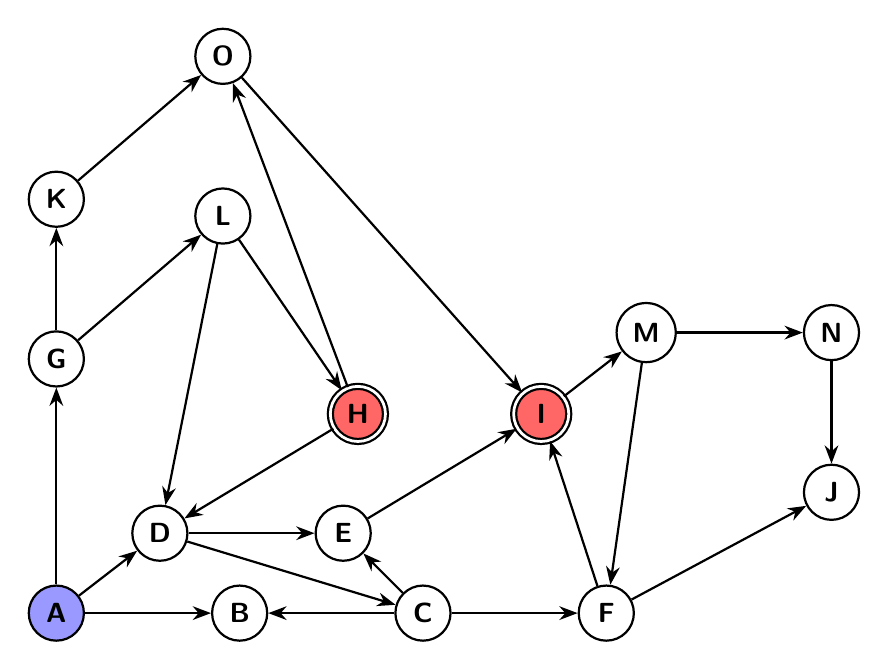
\begin{tikzpicture}[
	node distance=1.3cm and 1.6cm,
	every node/.style={circle, draw, thick, minimum size=7mm, font=\sffamily\bfseries},
	start_node/.style={fill=blue!40},
	goal_node/.style={fill=red!60, double, double distance=1pt},
	arrow/.style={-Stealth, thick}
	]
	
	% --- POSICIONAMENTO DOS NÓS (Layout da Figura 2) ---
	\node[start_node] (A) {A};
	\node[circle, draw] (G) [above=2.5cm of A] {G};
	\node[circle, draw] (K) [above=of G] {K};
	
	\node[circle, draw] (D) [above right=0.5cm and 0.8cm of A] {D};
	\node[circle, draw] (B) [right=of A] {B};
	\node[circle, draw] (L) [above right=of G] {L};
	
	\node[goal_node] (H) [above right=1cm and 2cm of D] {H};
	\node[circle, draw] (E) [above right=0.5cm and 0.8cm of B] {E};
	\node[circle, draw] (O) [above=of L] {O}; 
	
	\node[goal_node] (I) [right=of H] {I};
	\node[circle, draw] (C) [right=of B] {C};
	\node[circle, draw] (M) [above right=0.5cm and 0.8cm of I] {M};
	
	\node[circle, draw] (F) [right=of C] {F};
	\node[circle, draw] (N) [right=of M] {N};
	\node[circle, draw] (J) [below=of N] {J};
	
	\draw[arrow] (A) -- (G);
	\draw[arrow] (A) -- (D);
	\draw[arrow] (A) -- (B);
	
	\draw[arrow] (G) -- (K);
	\draw[arrow] (G) -- (L);
	
	\draw[arrow] (K) -- (O);
	\draw[arrow] (L) -- (H);
	\draw[arrow] (L) -- (D);
	

	\draw[arrow] (H) -- (O); 
	\draw[arrow] (H) -- (D);
	\draw[arrow] (O) -- (I); 
	
	\draw[arrow] (D) -- (E);
	\draw[arrow] (D) -- (C);
	
	\draw[arrow] (C) -- (B);
	\draw[arrow] (C) -- (E);
	\draw[arrow] (C) -- (F);
	\draw[arrow] (E) -- (I);
	
	\draw[arrow] (I) -- (M);
	\draw[arrow] (F) -- (I);
	\draw[arrow] (F) -- (J);
	\draw[arrow] (M) -- (N);
	\draw[arrow] (M) -- (F);
	\draw[arrow] (N) -- (J);
	
\end{tikzpicture}

Figura 2. Espaço de estados.


\subsection*{Resposta:}

\bigskip

\textbf{A)} Em uma busca em árvore, não há verificação de estados repetidos. A árvore termina quando um nó é uma meta (H ou I) ou quando não há sucessores.

\begin{forest}
	for tree={
		circle, draw, thick, minimum size=7mm,
		edge={-Stealth, thick},
		l sep=1cm, s sep=0.8cm
	}
	[A, fill=blue!30
	[B] % B agora é terminal
	[D
	[C
	[B]
	[E [I, double, fill=red!30]]
	[F [I, double, fill=red!30] [J]]
	]
	[E [I, double, fill=red!30]]
	]
	[G
	[K [O [I, double, fill=red!30]]]
	[L
	[D [C [B] [E [I, double, fill=red!30]] [F [I, double, fill=red!30] [J]]] [E [I, double, fill=red!30]]]
	[H, double, fill=red!30]
	]
	]
	]
\end{forest}

\newpage

\textbf{B)} 

\textbf{4.1) Busca em largura em árvore}

A árvore é expandida de forma completa nível por nível até que a meta H ou I seja extraída da borda.
Os estados repetidos aparecem como novos nós. Como a ordem de geração é alfabética e a busca é em largura, todos os nós de um nível são explorados antes de passar para o próximo.

\begin{forest}
	for tree={
		circle, draw, thick, minimum size=8mm,
		edge={-Stealth, thick},
		l sep=0.8cm, s sep=0.4cm,
		font=\sffamily\bfseries
	}
	[A, label={above:\textbf{1}} , fill=blue!30
	[B, label={above left:\textbf{2}}]
	[D, label={above right:\textbf{3}}
	[C, label={left:\textbf{5}}
	[B, label={below:\textbf{9}}]
	[E, label={below:\textbf{10}}]
	[F, label={below:\textbf{11}}]
	]
	[E, label={left:\textbf{6}}
	[I, label={below:\textbf{12}}, double, fill=red!30]
	]
	]
	[G, label={above right:\textbf{4}}
	[K, label={right:\textbf{7}}
	[O, label={below:\textbf{13}}]
	]
	[L, label={right:\textbf{8}}
	[D, label={below:\textbf{14}}]
	[H, label={below:\textbf{15}}, double, fill=red!30]
	]
	]
	]
\end{forest}

A busca só vai até o 12 e retorna o I. O restante é apenas a expansão, a consulta para na primeira meta encontrada.\\

\textbf{4.2)  Busca em largura em grafo}

O algoritmo mantém um conjunto de estados explorados. Um nó não é adicionado à borda se o estado já tiver sido visitado ou se já estiver na borda.

\begin{forest}
	for tree={
		circle, draw, thick, minimum size=8mm,
		edge={-Stealth, thick},
		l sep=1cm, s sep=0.6cm,
		font=\sffamily\bfseries
	}
	[A, label={above:\textbf{1}}, fill=blue!30
	[B, label={above left:\textbf{2}}]
	[D, label={above:\textbf{3}}
	[C, label={left:\textbf{5}}
	% B já foi visitado, E já está na borda (através de D)
	[F, label={below:\textbf{9}}]
	]
	[E, label={left:\textbf{6}}
	[I, label={below:\textbf{10}}, double, fill=red!30]
	]
	]
	[G, label={above right:\textbf{4}}
	[K, label={right:\textbf{7}}
	[O, label={below:\textbf{11}}]
	]
	[L, label={right:\textbf{8}}
	[H, label={below:\textbf{12}}, double, fill=red!30]
	% D já foi visitado
	]
	]
	]
\end{forest}

A busca só vai até o 10 e retorna o I. O restante é apenas a expansão, a consulta para na primeira meta encontrada.\\

\textbf{4.3)  Busca em profundidade em árvore}

O algoritmo explora o ramo mais à esquerda até o fim antes de fazer o backtracking. Não há memória de estados visitados.

\begin{forest}
	for tree={
		circle, draw, thick, minimum size=8mm,
		edge={-Stealth, thick},
		l sep=1cm, s sep=1cm,
		font=\sffamily\bfseries
	}
	[A, label={above:\textbf{1}}, fill=blue!30
	[B, label={below:\textbf{2}}] % B é terminal, faz backtracking
	[D, label={above right:\textbf{3}}
	[C, label={left:\textbf{4}}
	[B, label={below:\textbf{5}}] % Visita B novamente (em árvore pode)
	[E, label={left:\textbf{6}}
	[I, label={below:\textbf{7}}, double, fill=red!30] % META!
	]
	[F, label={below:não visitado}]
	]
	[E, label={right:não visitado}]
	]
	[G, label={right:não visitado}]
	]
\end{forest}\\

\textbf{4.4)  Busca em profundidade em grafo}

O algoritmo utiliza uma lista de estados explorados. Quando um nó é gerado, se o seu estado já foi visitado ou já está na borda, ele é descartado. O nó B não será visitado uma segunda vez quando a busca estiver explorando os filhos de C.

\begin{forest}
	for tree={
		circle, draw, thick, minimum size=8mm,
		edge={-Stealth, thick},
		l sep=1cm, s sep=1.2cm,
		font=\sffamily\bfseries
	}
	[A, label={above:\textbf{1}}, fill=blue!30
	[B, label={below:\textbf{2}}] % B visitado e adicionado aos explorados
	[D, label={above right:\textbf{3}}
	[C, label={left:\textbf{4}}
	% B aqui é ignorado pois já está no set de explorados
	[E, label={left:\textbf{5}}
	[I, label={below:\textbf{6}}, double, fill=red!30] % META!
	]
	[F, label={right:não visitado}]
	]
	[E, label={right:está na borda}] % E foi gerado por D e C, mas explorado via C
	]
	[G, label={right:não visitado}]
	]
\end{forest}\\

\textbf{4.5)  Busca de profundidade iterativa (passo da profundidade = 1) em grafo}

O algoritmo realiza múltiplas buscas em profundidade (DFS) com limites crescentes.\\

Casos de falha:

% Iteração L=0
\begin{forest}
	for tree={circle, draw, thick, minimum size=7mm}
	[A, label={right:\textbf{1 (L=0)}}, fill=blue!30]
\end{forest}

% Iteração L=1
\begin{forest}
	for tree={circle, draw, thick, minimum size=7mm, edge={-Stealth}}
	[A, label={above:\textbf{1 (L=1)}}, fill=blue!30
	[B, label={below:2}]
	[D, label={below:3}]
	[G, label={below:4}]
	]
\end{forest}

% Iteração L=2
\begin{forest}
	for tree={circle, draw, thick, minimum size=7mm, edge={-Stealth}, l sep=1cm, s sep=1cm}
	[A, label={above:\textbf{1 (L=2)}}, fill=blue!30
	[B, label={below:2}]
	[D, label={above:3}
	[C, label={below:4}]
	[E, label={below:5}]
	]
	[G, label={above:6}
	[K, label={below:7}]
	[L, label={below:8}]
	]
	]
\end{forest}\\

Caso de sucesso:

\begin{forest}
	for tree={
		circle, draw, thick, minimum size=8mm,
		edge={-Stealth, thick},
		l sep=1.1cm, s sep=1.2cm,
		font=\sffamily\bfseries
	}
	[A, label={above:\textbf{1 (L=3)}}, fill=blue!30
	[B, label={below:\textbf{2}}]
	[D, label={above right:\textbf{3}}
	[C, label={left:\textbf{4}}
	[E, label={left:\textbf{5}}
	[I, label={below:\textbf{6}}, double, fill=red!30] % Meta encontrada no Limite 3
	]
	[F, label={right:não visitado}]
	]
	[E, label={right:não visitado}]
	]
	[G, label={right:não visitado}]
	]
\end{forest}



\newpage
\section*{Exercício 10}

Considere o problema de cálculo de rotas entre diferentes cidades. No grafo ilustrado
da Figura 3, cada nó representa uma cidade distinta, e cada aresta, uma rodovia que
interliga duas cidades, cujo peso indica a distância, em km, entre essas cidades pepor
uma rodovia. Suponha que se deseje encontrar a melhor rota entre as cidades A e M,
indicadas nesse grafo. Considere, ainda, os valores indicados na tabela abaixo como a
distância em linha reta, em km, de cada cidade para a cidade M.


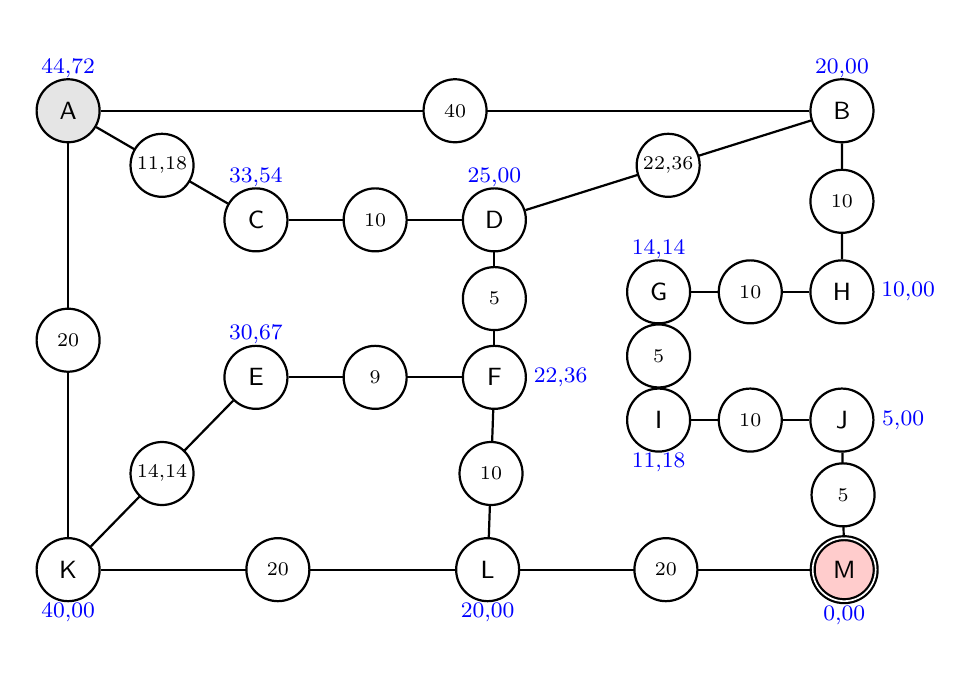
\begin{tikzpicture}[
	node distance=1.5cm and 2.2cm,
	every node/.style={circle, draw, thick, minimum size=8mm, font=\sffamily\small},
	heuristic/.style={draw=none, fill=none, font=\footnotesize\color{blue}, node distance=0.4cm},
	edge_label/.style={pos=0.5, font=\scriptsize, fill=white, inner sep=1pt}
	]
	
	% --- NÓS E SUAS HEURÍSTICAS h(n) ---
	\node[fill=gray!20] (A) {A}; \node[heuristic, above=-0.4cm of A] {44,72};
	\node (B) [right=9cm of A] {B}; \node[heuristic, above=-0.4cm of B] {20,00};
	\node (C) [below right=0.8cm and 1.8cm of A] {C}; \node[heuristic, above=-0.4cm of C] {33,54};
	\node (D) [right=of C] {D}; \node[heuristic, above=-0.4cm of D] {25,00};
	\node (E) [below right=2.8cm and 1.8cm of A] {E}; \node[heuristic, above=-0.4cm of E] {30,67};
	\node (F) [right=of E] {F}; \node[heuristic, right=-0.1cm of F] {22,36};
	\node (G) [above right=0.5cm and 1.5cm of F] {G}; \node[heuristic, above=-0.4cm of G] {14,14};
	\node (H) [right=1.5cm of G] {H}; \node[heuristic, right=-0.1cm of H] {10,00};
	\node (I) [below=0.8cm of G] {I}; \node[heuristic, below=-0.4cm of I] {11,18};
	\node (J) [right=1.5cm of I] {J}; \node[heuristic, right=-0.1cm of J] {5,00};
	\node (K) [below=5cm of A] {K}; \node[heuristic, below=-0.4cm of K] {40,00};
	\node (L) [right=4.5cm of K] {L}; \node[heuristic, below=-0.4cm of L] {20,00};
	\node[double, fill=red!20] (M) [right=3.7cm of L] {M}; \node[heuristic, below=-0.3cm of M] {0,00};
	
	% --- ARESTAS E CUSTOS g(n) ---
	\draw[thick] (A) -- node[edge_label] {11,18} (C);
	\draw[thick] (A) -- node[edge_label] {20} (K);
	\draw[thick] (A) -- node[edge_label] {40} (B);
	\draw[thick] (C) -- node[edge_label] {10} (D);
	\draw[thick] (D) -- node[edge_label] {5} (F);
	\draw[thick] (D) -- node[edge_label]{22,36} (B);
	\draw[thick] (B) -- node[edge_label] {10} (H);
	\draw[thick] (K) -- node[edge_label] {14,14} (E);
	\draw[thick] (K) -- node[edge_label] {20} (L);
	\draw[thick] (E) -- node[edge_label] {9} (F);
	\draw[thick] (F) -- node[edge_label] {10} (L);
	\draw[thick] (L) -- node[edge_label] {20} (M);
	\draw[thick] (G) -- node[edge_label] {5} (I);
	\draw[thick] (G) -- node[edge_label] {10} (H);
	\draw[thick] (I) -- node[edge_label] {10} (J);
	\draw[thick] (J) -- node[edge_label] {5} (M);
	
\end{tikzpicture}


\subsection*{Resposta:}

\bigskip

1. (V) Utilizando o algoritmo A*, a rota entre A e M encontrada é ACDFLM e o custo do caminho é 56,18.\\

O algoritmo A* escolhe o nó que minimiza $f(n) = g(n) + h(n)$.\\
O custo real ($g$) do caminho $A \to C \to D \to F \to L \to M$ é: $11,18 + 10 + 5 + 10 + 20 = \mathbf{56,18}$.\\
Comparando com outras rotas (como via K ou via B), este caminho apresenta o menor custo acumulado e a heurística é consistente, garantindo que o A* encontre essa rota como a ótima.\\

2. (F) Utilizando a busca gulosa, a rota encontrada no problema acima é ACDFLM.\\

A busca gulosa expande o nó com o menor valor de heurística $h(n)$.\\
De A, vizinhos são: $B(h=20)$, $C(h=33,54)$, $K(h=40)$. Escolhe B.\\
De B, vizinhos são: $F(h=22,36)$, $H(h=10)$. Escolhe H.\\
De H, vizinhos são: $B(h=20)$, $G(14,14)$. Escolhe G.\\
De G, vizinhos são: $I(h=11,18)$. Escolhe I.\\
De I, vizinhos são: $J(h=5,00)$. Escolhe J.\\
De J, vizinhos são: $M(h=0,00)$. Escolhe M.\\
Assim a rota na busca gulosa é ABHGIJM.\\


3. (V) Utilizando-se a busca gulosa, a rota encontrada no problema acima é ABHGIJM.\\

Feito na 2.\\

4. (F) Para utilizar algoritmos de busca heurística, deve-se definir uma heurística que superestime o custo da solução.\\

É o contrário. Para garantir a otimalidade do A*, a heurística deve ser admissível, o que significa que ela nunca pode superestimar o custo real até a meta ($h(n) \leq h^*(n)$). \\

5. (F) O A* é um algoritmo ótimo e completo quando heurísticas admissíveis são utilizadas, independentemente se usamos busca em árvore ou em grafo.\\

A admissibilidade garante a otimalidade apenas na busca em árvore. Para busca em grafo, a admissibilidade não é suficiente para garantir a otimalidade. É necessário que a heurística seja consistente (ou que o algoritmo reabra nós fechados). \\

6. (V) O A* é um algoritmo ótimo e completo quando heurísticas consistentes são utilizadas, independentemente se usamos busca em árvore ou em grafo.\\

A consistência garante que o $f(n)$ nunca diminua ao longo de um caminho. Isso assegura que, ao expandir um nó pela primeira vez em um grafo, o caminho encontrado até ele já é o ótimo.\\

7. (V) No algoritmo simulated annealing, é possível haver movimentos para um estado com avaliação pior do que a do estado corrente, dependendo da temperatura do processo e da probabilidade.\\

É um algoritmo de busca local projetado para escapar de máximos ou mínimos locais (pontos onde o algoritmo ficaria preso por não encontrar vizinhos melhores imediatos).\\

8. (F) Toda heurística admissível é consistente.\\

O inverso é verdadeiro (toda heurística consistente é admissível). Existem heurísticas que nunca superestimam o custo (admissíveis), mas que violam a desigualdade triangular entre nós sucessores, não sendo, portanto, consistentes.



\newpage
\section*{Exercício 13}

Considere duas heurísticas admissíveis h1(s) e h2(s). Prove que cada
uma das seguintes heurísticas induzidas a partir delas é admissível ou forneça um contraexemplo
caso não seja verdadeiro. Se necessário denote o custo exato à meta a partir de um
estado s por h* (s) e assuma que toda ação possui custo positivo.\\

a) $h_1 + h_2$\\
b) $h_1 \times h_2$\\
c) $max\{h_1, h_2\}$\\
d) $1 + min\{h_1, h_2\}$\\
e) $\alpha \times h_1 + \beta \times h_2,$ com $\alpha \geq 0$, $\beta \geq 0$ e $\alpha + \beta = 1$\\


\subsection*{Resposta:}

\bigskip


a) $h_1 + h_2$\\

Não é admissível.

\begin{proof}
Considere um estado $s$ onde o custo real até a meta é $h^*(s) = 10$. \\
Suponha $h_1(s) = 6$ e $h_2(s) = 7$. \\
Ambas são admissíveis individualmente ($6 \leq 10$ e $7 \leq 10$), mas a soma resulta em $h_1(s) + h_2(s) = 13$, o que supera o custo real $h^*(s) = 10$, violando a admissibilidade. \\
\end{proof}

b) $h_1 \times h_2$\\

Não é admissível.  

\begin{proof}
Se $h^*(s) = 5$, $h_1(s) = 2$ e $h_2(s) = 3$ (ambas admissíveis), o produto é $h_1 \times h_2 = 6$. \\
Como $6 > 5$, a heurística superestima o custo real e não é admissível.\\
\end{proof} 

c) $\max\{h_1, h_2\}$\\

É admissível.

\begin{proof}
Sabemos que $h_1(s) \leq h^*(s)$ e $h_2(s) \leq h^*(s)$, por definição de admissibilidade. \\
O valor máximo entre dois números que são ambos menores ou iguais a um terceiro, obrigatoriamente também será menor ou igual a esse terceiro: $\max\{h_1(s), h_2(s)\} \leq h^*(s)$. \\
\end{proof}  

d) $1 + \min\{h_1, h_2\}$\\

Não é admissível.

\begin{proof}
No estado meta $g$, por definição, o custo real é $h^*(g) = 0$ e qualquer heurística admissível deve retornar $h(g) = 0$.\\
Para esta função, teríamos $1 + \min\{0, 0\} = 1$. \\
Como $1 > 0$, ela superestima o custo no estado meta e falha na admissibilidade.\\
\end{proof}  

e) $\alpha \times h_1 + \beta \times h_2$, com $\alpha, \beta \geq 0$ e $\alpha + \beta = 1$\\

É admissível.

\begin{proof}
Esta é uma média ponderada de duas funções admissíveis. \\
Como $h_1(s) \leq h^*(s)$ e $h_2(s) \leq h^*(s)$, temos:\\
$$\alpha \times h_1(s) + \beta \times h_2(s) \leq \alpha \times h^*(s) + \beta \times h^*(s)$$ $$(\alpha + \beta) \times h^*(s) = 1 \times h^*(s) = h^*(s)$$ \\
Como o resultado é sempre menor ou igual a $h^*(s)$, a combinação permanece admissível. \\
\end{proof} 


\end{document}
